\documentclass[final_project_1.tex]{subfiles}
\begin{document}
\paragraph{}
Empirical process theory focus on the distribution of the realization of unknown underlying distribution. With this approach, we can throw away the structural assumption on the distribution, making the theory highly suitable for non-parametric statistical inference.
\subsection{Empirical Distribution}
\paragraph{}
As observers, all we can see from a random experiment is the sampling results from an underlying distribution (if there exists one). In almost every case, we don't know the true probability distribution behind it. What we want to do is to make inferences about the underlying distribution.

\subsubsection{Definition and Properties}
\paragraph{}
As long as we only have the samples, it's intuitively to make a histogram and observe the structure. Furthermore, we can consider the {\it empirical distribution function}
$$\hat{F}_n(x):=\frac{1}{n}\sum^{n}_{i=1}{\bf I}_{\{X_i\leq x\}}$$

where $X_1, X_2, ..., X_n$ are i.i.d. sample from a cumulative distribution function $F$. And ${\bf I}$ is the indicator function.

The intuition is that we record the number of occurrences from small sample value to large sample value and draw a cumulative function.

\paragraph{}
Also, we define {\it empirical process} according to the empirical distribution,
$$E_n(x):=\sqrt{n}[\hat{F}_n(x)-F(x)],\quad 0\leq x\leq 1$$
We will discuss more details about empirical process later. For now, let's observe some properties about empirical distribution.

\paragraph{}
The most important issue after defining the empirical distribution is to find out whether it will converge to the real underlying distribution. And first, we need to know what kind of convergence we are looking for. Point-wise convergence is the most basic convergence, and in the following part of this section will show you the result. To go further, we need some stronger results in the convergence of empirical distribution, so that we can construct something like confidence interval, which can be utilized in many applications.



\paragraph{}
As a warm-up, let's consider the point-wise convergence of empirical distribution to the underlying distribution: 
$$\hat{F}_n(z)\xrightarrow{P}F(z)$$ 
where $z\in [0,1]$

\paragraph{}
The point-wise convergence is an immediate result of the following observation.
\begin{observation}
The distribution of $n\hat{F}_n(z)$ for some $z\in\mathcal{R}$ is the same as $binomial(n, F(z))$. \end{observation}
You can look deep into figure 1 to find more intuition. And the point-wise convergence can be easily deduced.
\begin{figure}[h]
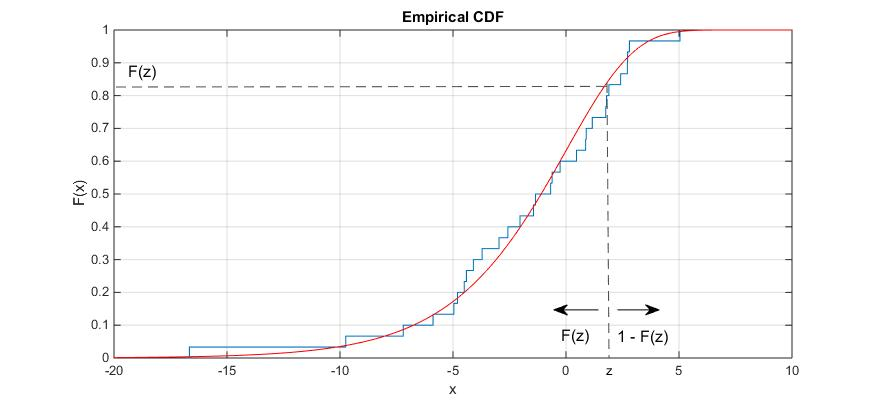
\includegraphics[scale=0.4]{empiricaldistribution_1.jpg}
\caption{Empirical distribution and its point-wise convergence property.}
\end{figure}

\begin{theorem}[Point-wise Convergence of Empirical Distribution]
Let $\hat{F}_n$ as the empirical distribution defined above from an underlying distribution $F$. Then $\forall z\in [0,1]$, 
$$\hat{F}_n(z)\xrightarrow{P}F(z)$$.
\end{theorem}

\begin{proof}
First, because $n\hat{F}_n(z)\sim binomial(n,F(z))$
\begin{align*}
E[\hat{F}_n(z)-F(z)] &= E[\hat{F}_n(z)] = F(z)\\
&=\frac{1}{n}E[n\hat{F}_n(z)]-F(z)\\
&=\frac{nF(z)}{n}-F(z) = 0
\end{align*}
Thus $\hat{F}_n$ is an unbiased estimator of $F$. Also, consider the variance
\begin{align*}
Var[\hat{F}_n(z)] &= \frac{1}{n^2}Var[n\hat{F}_n]\\
&=\frac{nF(z)[1-F(z)]}{n^2} = \frac{F(z)[1-F(z)]}{n}
\end{align*}
Applying Chebyshev inequality will lead to the result: $\hat{F}_n(z)\xrightarrow{P}F(z)$.
\end{proof}

\paragraph{}
Now we have the point-wise convergence of empirical distribution and the corresponding asymptotic rate. Based on this, we can construct confidence interval for point-wise estimation. For example, the ($1-\alpha$)-level confidence interval of $F(z)$ is
$$\hat{F}_n(z) \pm z_{\alpha/2}\sqrt{\frac{\hat{F}_n(z)[1-\hat{F}_n(z)]}{n}}$$
where $z_{\alpha/2}$ is half the size of the ($1-\alpha$)-level confidence interval of standard Gaussian random variable.

\paragraph{}
However, what if we want to estimate the behaviour of two points or an interval? We need a stronger results about the asymptotic behaviour of empirical distribution so that we can make effective inferences.

As a result, our goal is to understand the global asymptotic behaviour of empirical distribution. And we can see that, the global convergence behaviour can be controlled by the supremum norm. In other words, to prove the asymptotic behaviour of the empirical process, it's sufficient to show that of the supremum norm of it. Namely, the Kolmogorov Statistics of the empirical process. In the following section, we will introduce you the Uniform Law of Large Number(ULLN) and the Uniform Central Limit Theorem(UCLT) of empirical process. Then, we can yield the similar asymptotic convergence behaviour as in the traditional setting.

\begin{goal}[Uniform Convergence of Empirical Distribution]
The empirical distribution $E_n$ will converge in distribution to the underlying distribution.

\end{goal}

\subsubsection{Kolmogorov Statistics}
\paragraph{}
The Kolmogorov statistics is defined on an empirical distribution function $\hat{F}_n$ and a cumulative objective function $F$ as follow:
$$D_n:=\sup_{x\in\mathcal{R}}|\hat{F}_n(x)-F(x)|$$
where $n$ is the number of samples.

We can see that the Kolmogorov statistics $D_n$ is the supremum over empirical process $E_n$ defined in the previous subsection. The smaller the $D_n$ is we can some how think of that the closer the two distribution are.

As long as we consider the Kolmogorov statistics between the empirical distribution and its underlying distribution, there are some nice convergence behaviours.

\paragraph{}
The first one is {\it distribution-free property}. It means that no matter what underlying property is, the behaviour of the Kolmogorov statistics will be the same! Concretely, the distribution will only in some sense related to the uniform distribution.

\begin{theorem}[Distribution-Free Property]
The distribution of the Kolmogorov statistics $D_n$ is the same for all continuous underlying cumulative distribution.
\end{theorem}

\begin{proof}
For the simplicity, let's consider the case where $F$ is strictly increasing. Namely, $F^{-1}$ exists. Thus, $\forall x \in \mathcal{R}, \exists y\in[0,1]\ s.t.\ x=F(y)$. Consider the Kolmogorov statistics:
\begin{align*}
D_n&=\sup_{x\in\mathcal{R}}|\hat{F}_n(x)-F(x)| = \sup_{y\in[0,1]}|\hat{F}_n(F^{-1}(y))-F(F^{-1}(y))|\\
&=\sup_{y\in[0,1]}|\hat{F}_n(F^{-1}(y))-y|
\end{align*}
Observe the term $\hat{F}_n(F^{-1}(y))$
\begin{align*}
\hat{F}_n(F^{-1}(y))&=\frac{1}{n}\sum^{n}_{i=1}{\bf I}_{\{X_i\leq F^{-1}(y)\}}=\frac{1}{n}\sum^{n}_{i=1}{\bf I}_{\{F(X_i)\leq y\}}
\end{align*}
From Statistics101, we know that $F(X_i)$ has the same distribution as $Uni[0,1]$. As a result, the supremum will not differ from distribution to distribution. Actually, the distribution of $D_n$ will related to that of the ordered statistics of uniform distribution.
\end{proof}

Apart from the amazing fact that the distribution of Kolmogorov statistics is distribution-free, the convergence is also guaranteed by the following Glivenko-Cantelli theorem. Also, the asymptotic behaviour of Kolmogorov statistics is proved to be the same as the distribution of Brownian Bridge in another important theorem: Donsker Theorem. Both theorems will be discussed in details in the following subsection, and the definition and properties of Brownian Bridge will also be introduced in the Gaussian Process section.


\subsection{Asymptotic Convergence}
\paragraph{}
Our goal is to use empirical distribution to draw inference on the unknown. In the first part of the section we proved the point-wise convergence. In this part, we are going to explore two stronger results: Uniform Law of Large Number(ULLN) and Uniform Central Limit Theorem(UCLT).
\subsubsection{Glivenko-Cantelli Theorem: ULLN}
\paragraph{}
ULLN consider the universal convergence of the empirical distribution. And we can see that the convergence of Kolmogorov statistics, the supremum difference, is sufficient for the result. And it's guaranteed by the following Glivenko-Cantelli Theorem.
\begin{theorem}[Glivenko-Cantelli]
The Kolmogorov statistics will converge to zero almost surely as the number of samples grows to infinity. That is,
$$D_n\xrightarrow{a.s.}0$$, as $n\rightarrow\infty$
\end{theorem}

\begin{proof}
First, we consider the {\it ordered statistics} of the samples: $X_{1:n}, X_{2:n}, ..., X_{n:n}$ instead of the sample itself: $X_1, X_2, ..., X_n$. And it immediately follows that,
$\hat{F}_n(X_{i:n})=\frac{i}{n}$. Thus, 
$$D_n=max_{1\leq i\leq n}|\hat{F}_n(X_{i:n})-F(X_{i:n})|=max_{1\leq i\leq n}|\frac{i}{n}-X_{i:n}|$$
Next, we use the two properties of the ordered statistics of uniform distribution:
\begin{enumerate}
\centering
\item[(i)] $max_{1\leq i\leq n}|X_{i:n}-E[X_{i:n}]|\rightarrow 0$
\item[(ii)]$max_{1\leq i\leq n}|\frac{i}{n}-E[X_{i:n}]|\rightarrow 0$
\end{enumerate}
Inequality (i) is the result after applying the extension of Chebyshev inequality: $P[|X-E(X)|>\epsilon]\leq\frac{E[|X-E(X)|^k]}{\epsilon^k}$ up to fourth moment. And inequality (ii) is just the result of LLN.\\
With triangle inequality and the above two results from ordered statistics, we can conclude that
$$max_{1\leq i\leq n}|X_{i:n}-\frac{i}{n}]|\rightarrow 0$$
Thus, $D_n$ will converge to 0 as $n$ grows to infinity.
\end{proof}

With this theorem, we have the uniform convergence of empirical distribution. Namely, for any $\epsilon > 0$ there exists a $N$ such that for all $n>N$, the underlying distribution will lies in the $\epsilon$-neighborhood of the empirical distribution.

\subsubsection{Donsker Theorem: UCLT}
\paragraph{}
Finally, we come to the most important theorem in empirical process theory: the {\it Donsker Theorem}. 
\begin{theorem}[Donsker]
Let $E_n(x)=\hat{F}_n(x)-F(x)$ be the empirical process of $F$, which is a cumulative distribution function. Then, $En(x)$ will converge in distribution to a Gaussian process: Brownian Bridge. Thus, the limit of the empirical process $G(x)$ can be written as $B(F(x))$, where $B$ is the standard Brownian Bridge.
\end{theorem}

\paragraph{}
With Donsker theorem, we can easily construct the confidence interval of the Kolmogorov statistics $D_n$. And actually this is what Kolmogorov-Smirov test is doing.

\paragraph{}
To understand why Donsker theorem works, we need to know more about the distribution of the order statistics of uniform distribution. Also, we have to learn some basic concepts about Gaussian process, which will be introduced in the next section. As a result, the proof of Donsker theorem will be left until the last section.

\begin{remark}
Formally, the function that can be applied to Donsker theorem is in the Skorokhod space.
\end{remark}

\end{document}